\section{GF2-S2数据集检索}

\subsection{检索原则}
\begin{frame}{检索原则}
    根据人工的难易程度, 按照时间, 质量, 位置, 依次筛选数据
    \begin{itemize}
        \item 时间: 考虑正负14天的数据
        \item 质量: 考虑制作数据集成本, 云雾覆盖率, 云雾分布等情况筛选
        \item 位置: 哨兵大, 高分小. 保证边界盒有交集
    \end{itemize}
    
    \textbf{实际操作中, 先对哨兵数据和高分2号数据时间质量两者做筛选. 在筛选后的优质数据中, 寻找时间空间位置的交集.}
\end{frame}

\subsection{哨兵数据}
\begin{frame}{哨兵数据检索}{不可用数据}
    \begin{figure}[!htbp]
        \centering
        \subfloat[\tiny 云覆盖严重]{\label{fig:0104a}
        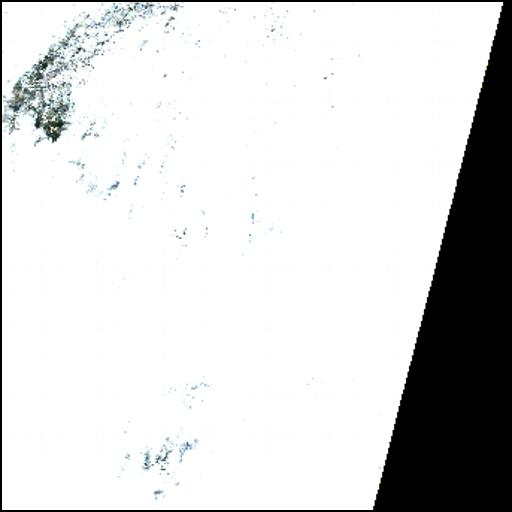
\includegraphics[width=4cm]{pic/pic0106.jpg}}
        \quad
        \subfloat[\tiny 可用数据过少]{\label{fig:0104b}
        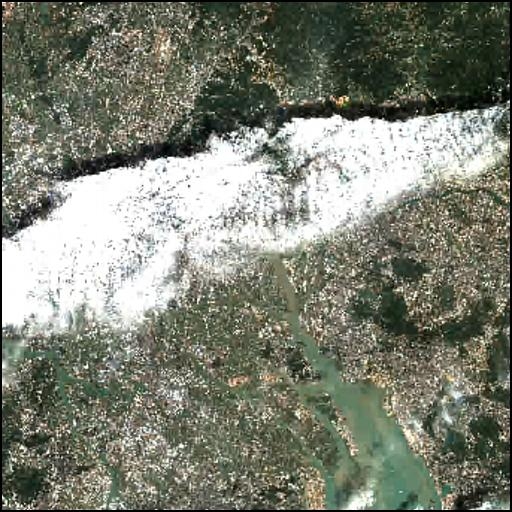
\includegraphics[width=4cm]{pic/pic0107.jpg}}
        \caption{云雾遮挡严重}
        \label{fig:0104}
    \end{figure}
\end{frame}

\begin{frame}{哨兵数据检索结果}
    \small 
    可用数据有以下:
    \begin{itemize}
        \item 一月: 0115, 0130
        \item 二月: 0221
        \item 三月: 0315
        \item 四月: 0409, 0429
        \item 十月: 1011, 1026
        \item 十一月: 1105, 1125, 1130
        \item 十二月: 1205, 1227, 1230
    \end{itemize}
\end{frame}

\subsection{高分2号数据}
\begin{frame}{高分2号数据时间筛选}    
    高分数据时间范围: 
    \begin{itemize}
        \item 2019年12月
        \item 2020年02, 04, 05, 07月
    \end{itemize}
    
    \vspace*{1cm}
    排除无可用哨兵影像的5月-9月

    高分数据只需对以下数据进行检索:
    \begin{itemize}
        \item 2019年12月
        \item 2020年02月, 04月
    \end{itemize}
\end{frame}

\begin{frame}{高分2号数据质量筛选}    
    除去云雾覆盖较为严重的影像:
    \small{除了完全无云雾的影像, 云雾分布集中一侧的也可使用}:
    \begin{figure}[!htbp]
        \centering
        \subfloat[\tiny 云雾覆盖]{\label{fig:0108a}
        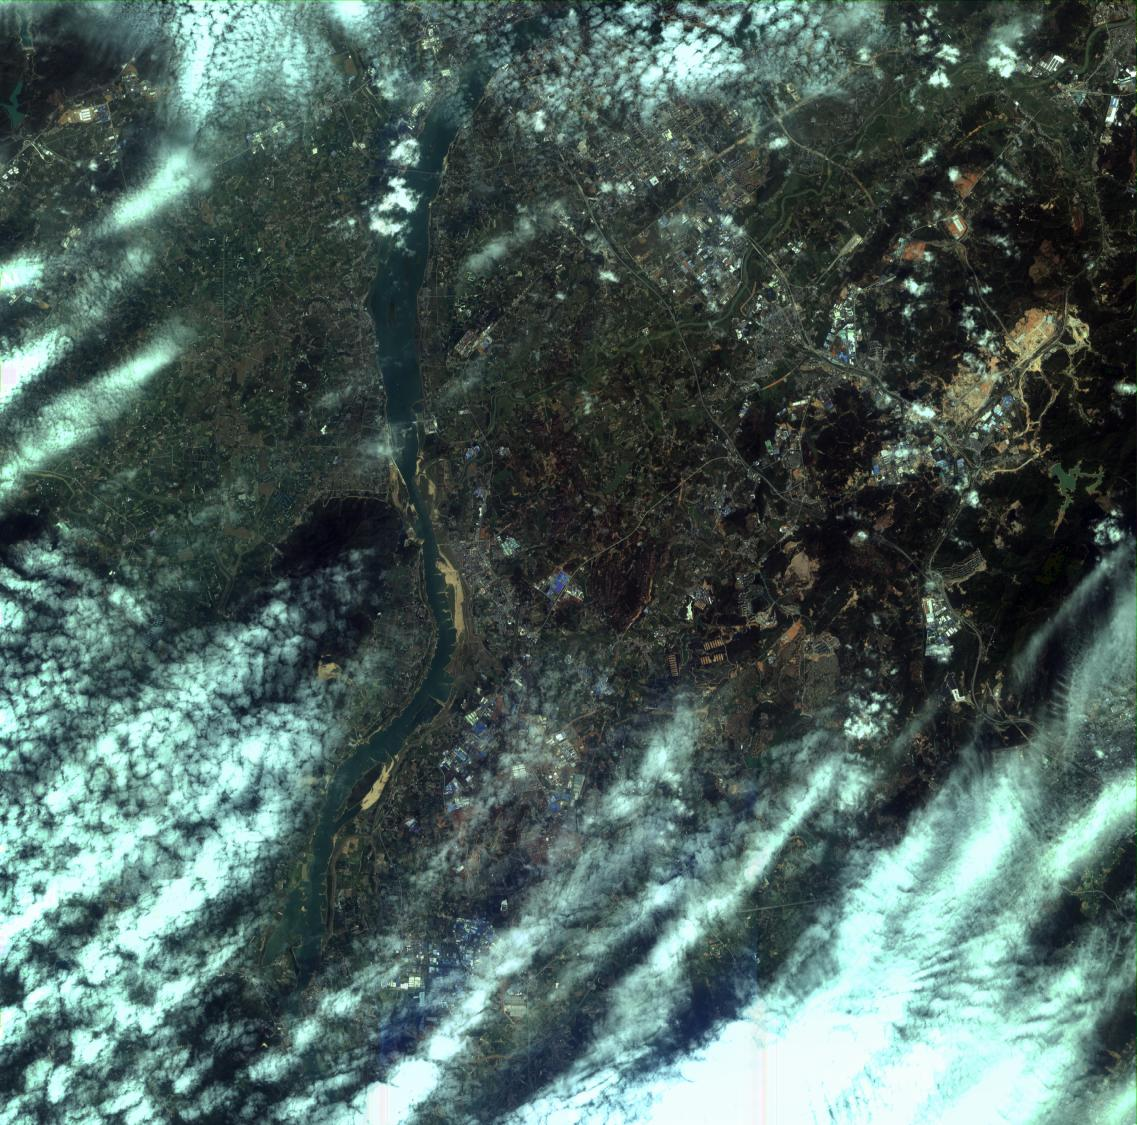
\includegraphics[width=4cm]{pic/pic0112.jpg}}
        \quad
        \subfloat[\tiny 云雾覆盖]{\label{fig:0108b}
        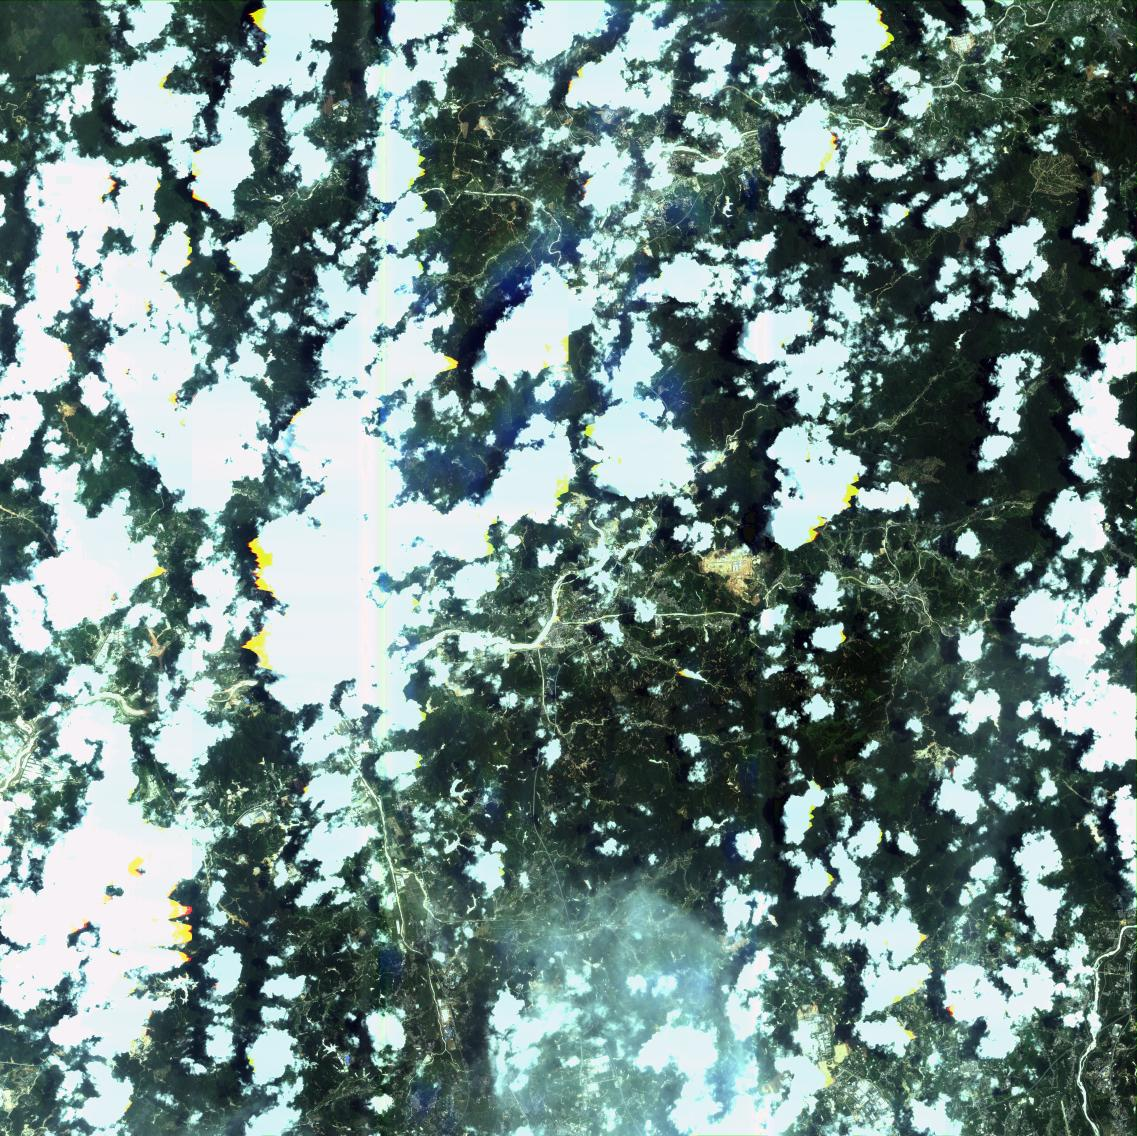
\includegraphics[width=4cm]{pic/pic0113.jpg}}
        \caption{云雾覆盖严重}
        \label{fig:0108}
    \end{figure}
\end{frame}

\subsection{检索结果}
\begin{frame}{数据集1}
    \small 哨兵数据为
    
    \begin{itemize}
        \item 20191226T030129N0213R032T49QGF
    \end{itemize}
    \small 高分2号数据为

    \begin{itemize}
        \item E113.1N22.820191227L1A0004731172
        \item E113.1N23.020191227L1A0004507320
        \item E113.2N23.320191227L1A0004507303
        \item E113.3N22.820191227L1A0004505423
        \item E113.3N22.920191227L1A0004505422
        \item E113.4N23.120191227L1A0004505416
    \end{itemize}
\end{frame}

\begin{frame}{数据集2}
    \tiny
    哨兵数据为
    \begin{itemize}
        \item 20200429T025551N0214R032T49QGF
        \item 20200429T025551N0214R032T49QGG
        \item 20200429T025551N0214R032T49QKM
    \end{itemize}
    高分2号数据为
    
    \begin{itemize}
        \item E113.8N23.120200428L1A0004767988
        \item E113.8N23.320200428L1A0004767982
        \item E113.9N23.520200428L1A0004767976
        \item E113.9N23.720200428L1A0004768005
        \item E114.0N23.920200428L1A0004768001
        \item E113.9N22.820200428L1A0004768660
        \item E114.2N23.820200428L1A0004768656
    \end{itemize}
\end{frame}

\begin{frame}{最终结果}
    数据集1:
    \begin{figure}
        \centering
        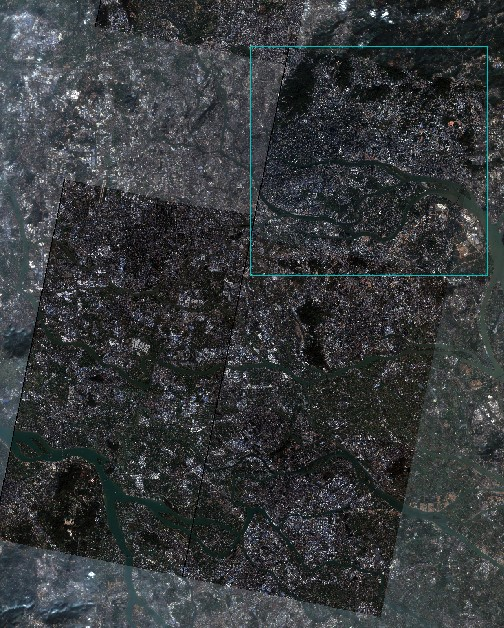
\includegraphics[height=5cm]{pic/pic0114.jpg}
        \caption{数据集1结果}
        \label{fig:0101}
    \end{figure}
\end{frame}